\chapter{Implementation and Compiler Engineering}
\label{ch:implementation}

\section{System Architecture Overview}
\label{sec:system_arch_overview}

Translating the abstract mathematics of algebraic topology and Clifford algebra into a high-throughput, low-latency execution system requires an optimizing compiler infrastructure. The \ToposLang{} compiler system bridges the semantic gap between high-level cellular declarations and physical hardware through a specialized Multi-Level Intermediate Representation (MLIR) dialect named \texttt{topos} \cite{lattner2021mlir}.

This chapter details the engineering architecture of the \ToposLang{} compiler and runtime:
\begin{enumerate}[leftmargin=1.5cm]
    \item The specification of the \texttt{topos} MLIR dialect, its types, operations, and C++ static verifiers;
    \item The exact rational linear algebra engine over $\mathbb{Q}$, guaranteeing exact rank and Betti number computation;
    \item The \texttt{--topos-symbolic-gnc} optimization pass, which evaluates multivector products symbolically to eliminate the $O(2^{2n})$ blade penalty;
    \item The spatial support closure and lock-free wavefront scheduler algorithms;
    \item The memory management subsystem, featuring homology-preserving cellular garbage collection;
    \item Hardware compilation backends targeting multi-core CPUs, TPUs, and dedicated Clifford coprocessors.
\end{enumerate}

---

\section{The Topos MLIR Dialect Specification}
\label{sec:mlir_dialect}

\subsection{Dialect Types and C++ Memory Layouts}
The \texttt{topos} dialect introduces native dialect types modeling topological and geometric entities.

\subsubsection{1. Type \texttt{!topos.cell<dim: i32>}}
Represents a single, oriented $k$-dimensional topological cell $e^k \in K_k$.
\begin{lstlisting}[language=C++, caption={C++ Memory Layout for \texttt{!topos.cell}.}]
struct ToposCell {
    uint64_t cell_id;
    uint32_t dim;
    // Sparse mapping of boundary face cell IDs to orientation signs (+1 or -1)
    llvm::SmallDenseMap<uint64_t, int8_t, 4> boundary_faces;
};
\end{lstlisting}

\subsubsection{2. Type \texttt{!topos.chain<dim: i32, field: type>}}
Represents a formal linear combination of $k$-cells $c = \sum a_i e_i^k \in C_k(\mathcal{K}; \mathbb{F})$.
\begin{lstlisting}[language=C++, caption={C++ Memory Layout for \texttt{!topos.chain}.}]
struct ToposChain {
    uint32_t dim;
    // Map of cell IDs to exact rational coefficients or multivector coefficients
    llvm::SmallDenseMap<uint64_t, ExactRational, 8> coefficients;
};
\end{lstlisting}

\subsubsection{3. Type \texttt{!topos.complex<max\_dim: i32>}}
The state container for the Directed Acyclic Cell Complex $\mathcal{K} = (K, \partial)$.
\begin{lstlisting}[language=C++, caption={C++ Memory Layout for \texttt{!topos.complex}.}]
struct ToposComplex {
    uint32_t max_dim;
    // Graded cell arrays: cells_by_dim[k] contains all k-cells
    std::vector<std::vector<ToposCell>> cells_by_dim;
    // Sparse boundary incidence matrices B_k in CSR format
    std::vector<SparseMatrixCSR<ExactRational>> boundary_matrices;
};
\end{lstlisting}

\subsection{Dialect Operations}
The dialect defines operations for boundary mapping, homotopy rewriting, and support closures:

\begin{lstlisting}[language={}, caption={MLIR \texttt{topos} Dialect Operations.}]
// Compute boundary chain: c_out = B_k * c_in
%out_chain = topos.boundary %in_chain : !topos.chain<1, Q> -> !topos.chain<0, Q>

// Compute downward topological support closure
%supp_set = topos.support_closure %complex, %chain : !topos.complex<2>, !topos.chain<1, Q> -> !topos.set<cell>

// Test spatial disjointness between two support sets
%is_disjoint = topos.spatial_disjoint %supp_set_a, %supp_set_b : !topos.set<cell>, !topos.set<cell> -> i1

// Attach a higher-dimensional cell alpha to perform a homotopy state transition
%new_complex = topos.homotopy_rewrite %complex, %lhs_chain, %rhs_chain : 
    !topos.complex<2>, !topos.chain<1, Q>, !topos.chain<1, Q> -> !topos.complex<2>
\end{lstlisting}

\subsection{Static Verification Hooks: Boundary Nilpotency ($\partial^2 = 0$)}
The compiler guarantees structural safety by executing an axiomatic verifier hook before lowering the \texttt{topos.homotopy\_rewrite} operation:

\begin{lstlisting}[language=C++, caption={C++ Static Verifier Hook for Homotopy Rewrite Operations.}]
mlir::LogicalResult HomotopyRewriteOp::verify() {
    ToposChain lhs = this->getLhs();
    ToposChain rhs = this->getRhs();

    // 1. Verify topological dimensions match
    if (lhs.dim() != rhs.dim()) {
        return emitOpError("LHS and RHS must possess identical dimensions.");
    }

    // 2. Compute algebraic difference representing the boundary of the attaching cell
    ToposChain target_boundary = rhs - lhs;

    // 3. Axiomatic Verification: d(target_boundary) MUST equal zero
    ToposChain d_squared = computeBoundary(target_boundary);

    if (!d_squared.isZero()) {
        return emitOpError() << "Boundary Nilpotency Violation (d^2 != 0).\n"
                             << "The specified rewrite creates a non-closed geometric attachment.\n"
                             << "Residual boundary: " << d_squared;
    }

    return mlir::success();
}
\end{lstlisting}

\subsection{Static Verification Test Suite and Ground-Truth Invariants}
The compiler test harness validates the static verifier against three canonical geometric benchmarks:

\subsubsection{Test Case 1: Hollow Triangle (Topological Circle $S^1$)}
\begin{itemize}[leftmargin=1.5cm]
    \item \textbf{Geometry:} 3 Vertices ($v_0, v_1, v_2$), 3 Edges ($e_0, e_1, e_2$) forming a 1-cycle. No 2-cells.
    \item \textbf{Incidence Matrix $B_1 \in \mathbb{Q}^{3 \times 3}$:}
    \begin{equation}
        B_1 = \begin{bmatrix}
            -1 & 0 & -1 \\
            1 & -1 & 0 \\
            0 & 1 & 1
        \end{bmatrix}
    \end{equation}
    \item \textbf{Rank Analysis:} $\rank(B_1) = 2$.
    \item \textbf{Verified Invariants:} $\beta_0 = 3 - 2 = 1$ (one component), $\beta_1 = 3 - 2 - 0 = 1$ (one central cycle), $\chi = 3 - 3 = 0$.
\end{itemize}

\subsubsection{Test Case 2: Solid Triangle (2-Simplex)}
\begin{itemize}[leftmargin=1.5cm]
    \item \textbf{Geometry:} Same as Test 1, with one attached 2-cell ($f_0$) whose boundary is $e_0 + e_1 - e_2$.
    \item \textbf{Incidence Matrix $B_2 \in \mathbb{Q}^{3 \times 1}$:}
    \begin{equation}
        B_2 = \begin{bmatrix} 1 \\ 1 \\ -1 \end{bmatrix}
    \end{equation}
    \item \textbf{Nilpotency Check:}
    \begin{equation}
        B_1 B_2 = \begin{bmatrix}
            -1 & 0 & -1 \\
            1 & -1 & 0 \\
            0 & 1 & 1
        \end{bmatrix} \begin{bmatrix} 1 \\ 1 \\ -1 \end{bmatrix} = \begin{bmatrix} 0 \\ 0 \\ 0 \end{bmatrix} \quad (\text{Passes Axiom 1.1})
    \end{equation}
    \item \textbf{Verified Invariants:} $\beta_0 = 1$, $\beta_1 = 3 - 2 - 1 = 0$ (hole contracted), $\chi = 3 - 3 + 1 = 1$.
\end{itemize}

\subsubsection{Test Case 3: Disjoint Edges (Two Separate 1-Simplices)}
\begin{itemize}[leftmargin=1.5cm]
    \item \textbf{Geometry:} 4 Vertices ($v_0, v_1, v_2, v_3$), 2 Edges ($e_0 = [v_0, v_1]$, $e_1 = [v_2, v_3]$).
    \item \textbf{Incidence Matrix $B_1 \in \mathbb{Q}^{4 \times 2}$:}
    \begin{equation}
        B_1 = \begin{bmatrix}
            -1 & 0 \\
            1 & 0 \\
            0 & -1 \\
            0 & 1
        \end{bmatrix}, \quad \rank(B_1) = 2
    \end{equation}
    \item \textbf{Verified Invariants:} $\beta_0 = 4 - 2 = 2$ (two independent components), $\beta_1 = 2 - 2 = 0$, $\chi = 4 - 2 = 2$.
\end{itemize}


---

\section{Exact Rational Linear Algebra Engine}
\label{sec:exact_linear_algebra}

\subsection{Preventing Floating-Point Cancellation in Homology}
In numerical linear algebra, calculating matrix rank using standard floating-point Singular Value Decomposition (SVD) or QR decomposition introduces catastrophic failure when applied to topological invariants. Because Betti numbers are integers ($\beta_k \in \mathbb{N}$), rounding errors in floating-point pivots can falsely identify small singular values as non-zero, erroneously collapsing structural holes ($\beta_1 = 0$) or fabricating spurious topological features.

\paragraph{The Systems Why: Discrete Invariants vs. Continuous Approximations.}
In numerical physics, an error of $10^{-15}$ is negligible because physical measurements are continuous approximations. In algebraic topology, however, vector space dimension is an integer: a matrix column is either linearly independent or it is not. If an IEEE-754 rounding error produces a residual pivot of $1.4 \times 10^{-16}$ instead of $0.0$, an SVD or LU routine with an improper threshold will treat this pivot as non-zero. This increases the computed matrix rank by 1, instantly reducing the computed Betti number $\beta_1$ from 1 to 0. In an invariant control loop $\texttt{until betti(1) == 0}$, this numerical artifact triggers a \textit{premature loop termination}: the software believes an open transaction or deadlock has resolved when it has physically stalled.

To eliminate floating-point non-determinism, \ToposLang{} implements a dedicated \textbf{Exact Rational Linear Algebra Engine over $\mathbb{Q}$}. Rational numbers $q = a/b$ are stored as canonical pairs of arbitrary-precision integers $(a, b)$ with $\gcd(a, b) = 1$ and $b > 0$. Every pivot operation is mathematically exact, ensuring that computed topological invariants are completely immune to machine precision artifacts.

\subsection{Exact Reduced Row Echelon Form (RREF) Algorithm}
Matrix rank and null spaces are evaluated via exact Gaussian elimination over $\mathbb{Q}$:

\begin{lstlisting}[language=Python, caption={Exact Rational Reduced Row Echelon Form (RREF) Algorithm.}]
def rref_and_rank(matrix: MatrixQ) -> Tuple[MatrixQ, int]:
    """Computes exact Reduced Row Echelon Form and matrix rank over Q."""
    mat = matrix.copy()
    pivot_row = 0
    pivot_cols = []

    for col in range(mat.cols):
        if pivot_row >= mat.rows:
            break

        # Search for non-zero pivot entry in column `col`
        sel_row = -1
        for r in range(pivot_row, mat.rows):
            if mat[r, col] != Fraction(0, 1):
                sel_row = r
                break

        if sel_row == -1:
            # Column is all zeros; advances nullity without advancing pivot row
            continue

        # Swap pivot row into active position
        mat.data[pivot_row], mat.data[sel_row] = mat.data[sel_row], mat.data[pivot_row]

        # Normalize pivot row leading entry to 1
        pivot_val = mat[pivot_row, col]
        for c in range(mat.cols):
            mat[pivot_row, c] /= pivot_val

        # Eliminate all other non-zero entries in column `col`
        for r in range(mat.rows):
            if r != pivot_row and mat[r, col] != Fraction(0, 1):
                factor = mat[r, col]
                for c in range(mat.cols):
                    mat[r, c] -= factor * mat[pivot_row, c]

        pivot_cols.append(col)
        pivot_row += 1

    rank = len(pivot_cols)
    return mat, rank
\end{lstlisting}

\subsection{Combinatorial Hodge Laplacian and Invariant Spectra}
The Hodge Laplacian $L_k = B_k^T B_k + B_{k+1} B_{k+1}^T$ is formed via exact rational sparse matrix multiplication. The Betti numbers are computed directly from the exact ranks:
\begin{equation}
    \beta_k = |K_k| - \rank(B_k) - \rank(B_{k+1})
\end{equation}
Because every arithmetic step is exact over $\mathbb{Q}$, the computed Betti numbers are mathematically guaranteed to be free of numerical drift.

---

\section{Symbolic Optimization Engine: \texttt{--topos-symbolic-gnc}}
\label{sec:symbolic_gnc}

\subsection{The Multivector Dimensionality Barrier}
A primary challenge in implementing Clifford algebras is the exponential dimensionality of multivector spaces:
\begin{itemize}[leftmargin=1.5cm]
    \item 3D Projective Geometric Algebra ($\mathbb{R}^{3,0,1}$): $2^4 = 16$ dimensions;
    \item 3D Conformal Geometric Algebra ($\mathbb{R}^{4,1,0}$): $2^5 = 32$ dimensions;
    \item Space-Time Algebra ($\mathbb{R}^{1,3,0}$): $2^4 = 16$ dimensions.
\end{itemize}
A naive general multiplication of two 32-dimensional CGA multivectors requires $32 \times 32 = 1024$ scalar multiplications and additions. However, in physical geometric operations, most input entities are sparse blades possessing only a few non-zero components (e.g., a point or plane in PGA requires only 4 components).

\subsection{Compile-Time AST Expansion and Zero-Blade Pruning}
The \texttt{--topos-symbolic-gnc} optimization pass intercepts multivector operations in the AST and evaluates them symbolically before emitting LLVM IR:

\begin{figure}[h]
\centering
\small
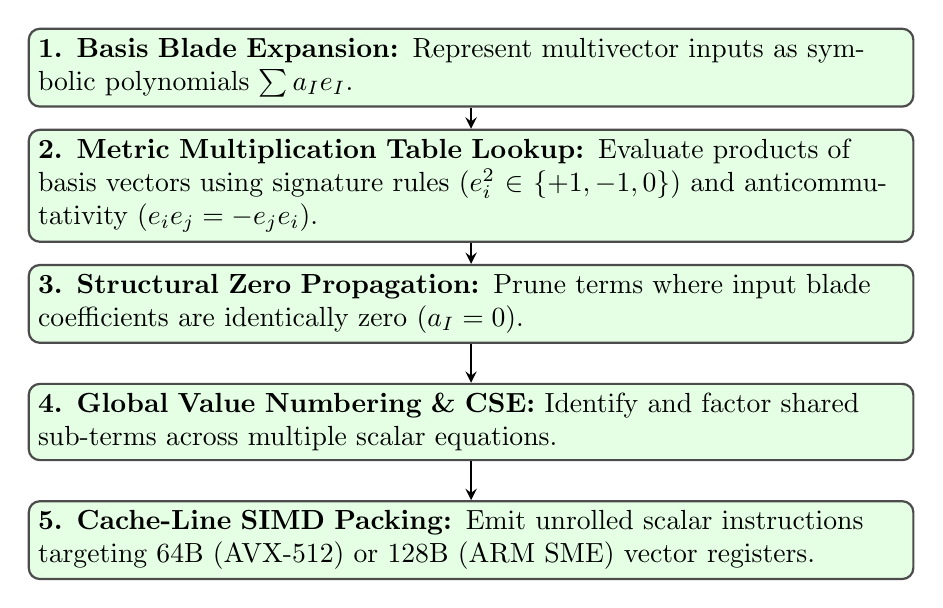
\begin{tikzpicture}[node distance=1.5cm, auto,
    proc/.style={rectangle, draw=black!70, fill=green!10, thick, text width=11cm, minimum height=0.9cm, rounded corners},
    flow/.style={thick, ->, >=stealth}]

    \node [proc] (p1) {\textbf{1. Basis Blade Expansion:} Represent multivector inputs as symbolic polynomials $\sum a_I e_I$.};
    \node [proc, below of=p1] (p2) {\textbf{2. Metric Multiplication Table Lookup:} Evaluate products of basis vectors using signature rules ($e_i^2 \in \{+1, -1, 0\}$) and anticommutativity ($e_i e_j = -e_j e_i$).};
    \node [proc, below of=p2] (p3) {\textbf{3. Structural Zero Propagation:} Prune terms where input blade coefficients are identically zero ($a_I = 0$).};
    \node [proc, below of=p3] (p4) {\textbf{4. Global Value Numbering \& CSE:} Identify and factor shared sub-terms across multiple scalar equations.};
    \node [proc, below of=p4] (p5) {\textbf{5. Cache-Line SIMD Packing:} Emit unrolled scalar instructions targeting 64B (AVX-512) or 128B (ARM SME) vector registers.};

    \draw [flow] (p1) -- (p2);
    \draw [flow] (p2) -- (p3);
    \draw [flow] (p3) -- (p4);
    \draw [flow] (p4) -- (p5);
\end{tikzpicture}
\caption{The Symbolic GNC Optimization Pipeline.}
\label{fig:symbolic_pipeline}
\end{figure}

For example, computing the sandwich transformation of a point $P = x e_{023} + y e_{031} + z e_{012} + w e_{123}$ by a motor $M = R + e_0 T$ in PGA reduces from 256 potential operations to exactly 28 floating-point scalar instructions, completely eliminating dynamic multivector allocation.

---

\section{Spatial Support Closures and Wavefront Scheduling}
\label{sec:wavefront_scheduler}

\subsection{Downward Support Closure Algorithm}
The spatial footprint of any formal chain is computed by recursively traversing the incidence graph down to dimension 0:

\begin{lstlisting}[language=Python, caption={Algorithm: Downward Support Closure Computation.}]
def compute_downward_closure(complex_store: DACC, chain: Chain) -> Set[str]:
    """Computes downward topological closure cl(c) down to 0-cells."""
    closure_set: Set[str] = set()
    worklist: List[str] = list(chain.coeffs.keys())

    while len(worklist) > 0:
        cell_id = worklist.pop()
        if cell_id in closure_set:
            continue
        closure_set.add(cell_id)
        cell = complex_store.cells[cell_id]
        if cell.dim > 0:
            for face_id in cell.boundary_faces.keys():
                if face_id not in closure_set:
                    worklist.append(face_id)

    return closure_set
\end{lstlisting}

\subsection{Lock-Free Wavefront Partitioning Algorithm}
Given a collection of pending rewrite rules $R = \{r_1, r_2, \dots, r_m\}$, the runtime scheduler partitions them into a sequence of concurrent execution wavefronts:

\begin{lstlisting}[language=Python, caption={Algorithm: Spatial Wavefront Partitioning.}]
def partition_into_wavefronts(rules: List[RewriteRule], complex_store: DACC) -> List[List[RewriteRule]]:
    """Partitions rules into concurrent wavefronts based on spatial disjointness."""
    # Precompute spatial support closures for all rules
    supports = {r: compute_downward_closure(complex_store, r.lhs).union(
                   compute_downward_closure(complex_store, r.rhs)) for r in rules}
    wavefronts: List[List[RewriteRule]] = []
    pending = list(rules)

    while len(pending) > 0:
        current_wavefront: List[RewriteRule] = []
        wavefront_support: Set[str] = set()

        for r in list(pending):
            r_supp = supports[r]
            # Spatial disjointness check
            if wavefront_support.isdisjoint(r_supp):
                current_wavefront.append(r)
                wavefront_support.update(r_supp)
                pending.remove(r)

        wavefronts.append(current_wavefront)

    return wavefronts
\end{lstlisting}

Each wavefront is dispatched across available hardware worker threads. Because all rules within a wavefront modify mutually disjoint memory addresses and sparse matrix columns, execution completes with **zero thread synchronization contention**.

---

\section{Topological Memory Architecture and Cellular Garbage Collection}
\label{sec:topological_gc}

\subsection{Cellular Garbage Collection via Homotopy Contractions}
In classical runtimes, garbage collection relies on reference counting or tracing mark-and-sweep passes, both of which suffer from cyclic reference deadlocks and stop-the-world latency spikes.

In \ToposLang{}, memory is a cell complex. Garbage collection is formalized as a **Topological Contraction (Collapsing)**. When intermediate computational history cells (e.g., intermediate attaching cells $\alpha_r$) are no longer referenced by active execution pointers, the runtime collapses them via elementary simplicial collapses \cite{kozlov2008combinatorial}:
\begin{definition}[Elementary Topological Collapse]
Let $e^{k-1}$ be a regular boundary face of a unique cell $e^k$ in complex $\mathcal{K}$. The pair $(e^{k-1}, e^k)$ forms a \textbf{free pair}. The elementary collapse is the topological deformation retract:
\begin{equation}
    \mathcal{K} \searrow \mathcal{K} \setminus \{ e^{k-1}, e^k \}
\end{equation}
\end{definition}
Elementary collapses are guaranteed by algebraic topology to strictly preserve all homology groups and Betti numbers:
\begin{equation}
    H_*(\mathcal{K} \setminus \{e^{k-1}, e^k\}) \cong H_*(\mathcal{K})
\end{equation}
The \ToposLang{} runtime performs cellular garbage collection by continuously contracting free pairs in inactive sub-complexes, reclaiming memory without modifying global invariants or requiring stop-the-world pauses.

\paragraph{The Systems Why: Eradicating the Cyclic Reference Problem.}
In classical object runtimes (such as CPython, Java, or Swift), when two objects point to each other in a cyclic dependency ($A \longleftrightarrow B$), naive reference-counting algorithms fail to reclaim memory because reference counters cannot reach zero. Runtimes are forced to execute expensive global mark-and-sweep or generational tracing passes, causing non-deterministic ``stop-the-world'' latency pauses.

In \ToposLang{}, cyclic relational structures are explicitly represented as 1-cycles (chains in $Z_1$). When a process contracts a transaction, the intermediate attaching cell and its uniquely incident boundary face form a \textit{free pair} in the complex. The runtime identifies free pairs locally in $O(1)$ time and collapses them simultaneously. Because this operation is purely local and mathematically proven to preserve global Betti numbers ($H_*(\mathcal{K}) \cong H_*(\mathcal{K}')$), cellular memory is reclaimed continuously without heap tracing, reference-counting overhead, or thread suspension.

---

\section{Hardware Acceleration and Dedicated Coprocessors}
\label{sec:hardware_coprocessors}

\subsection{Lowering to AI Tensor Accelerators (TPUs / GPUs)}
Because boundary operations in \ToposLang{} are represented by sparse incidence matrices $B_k$, parallel execution wavefronts lower directly to sparse tensor operations on Tensor Processing Units (TPUs) and GPUs:
\begin{itemize}[leftmargin=1.5cm]
    \item Boundary evaluations map to sparse matrix-dense vector multiplications ($\text{SpMV}$);
    \item Hodge Laplacians $L_k = B_k^T B_k + B_{k+1} B_{k+1}^T$ map to sparse matrix-matrix products ($\text{SpGEMM}$);
    \item Multi-agent wavefronts map to block-diagonal partitioned tensor kernels executing concurrently on independent tensor cores.
\end{itemize}

\subsection{Silicon Implementation: The CliffordALU Coprocessor Architecture}
For edge robotics and embedded spatial systems, \ToposLang{} targets dedicated silicon coprocessors:
\begin{itemize}[leftmargin=1.5cm]
    \item \textbf{CliffordALU5} \cite{breuils2013embedded}: An embedded FPGA/ASIC coprocessor implementing native hardware execution for up to 5-dimensional Clifford algebras. It utilizes hardware bit-manipulation tables to compute basis blade sign changes and grade projections in a single clock cycle.
    \item \textbf{ConformalALU} \cite{rodriguez2022optimized}: A pipelined FPGA System-on-Chip (SoPC) architecture containing dedicated motor transformation pipelines and outer wedge product intersection units, evaluating rigid body kinematics and collision queries at ultra-low latency.
\end{itemize}
The \ToposLang{} backend emits direct hardware instruction words for these coprocessors, achieving orders-of-magnitude energy efficiency improvements over general-purpose CPUs.
